\documentclass[../main.tex]{report}

\begin{document}

\theoremstyle{plain}
\newtheorem{Thm}{Théorème}

\subsection{Approche analytique}

Cette approche pour créer des ensembles aléatoires (désignés par $Q$) qui partagent la même distribution que celle des nombres
premiers, est basée sur un théorème (théorème \ref{theorem}) issu de ... . 

\begin{Thm}
\label{theorem}
	L'hypothèse de Reimann est équivalente à l'assertion 
	\[
	\forall \ n \geqslant 11, \ |p_{n} - ali(n) | < \frac{1}{\pi} \sqrt{n} \log^{5/2}(n) 
	\]
	où $p_{n}$ représente le n-ième nombre premier.
\end{Thm}

\subsubsection{Méthode de création d'un ensemble aléatoire $Q$}

Les onze premiers éléments d'un ensemble $Q$ sont choisis arbitrairement. 
Pour $ n > 11 $, voici la méthode de sélection  de l'élément $q_{n} \in Q$: 
\begin{itemize}
	\item on pose $ a = \max \left\{ q_{n-1} ,\lceil{ali(n) - \frac{1}{\pi} \sqrt{n} \log^{5/2}(n) \rceil} \right\}$ 
	(où $\lceil x \rceil$ désigne la partie entière supérieure de $x$);
	\item on pose $ b = \lfloor ali(n) + \frac{1}{\pi} \sqrt{n} \log^{5/2}(n) \rfloor $
	(où $\lfloor x \rfloor$ désigne la partie entière inférieure de $x$);
	\item $ q_{n} $ est choisi aléatoirement entre a et b. 
\end{itemize}
En procédant de la sorte, le théorème \ref{theorem} sera toujours vrai pour tout ensemble aléatoire $Q$.

\subsubsection{Définition de la fonction $\sigma$}

On peut désormais définir $ \sigma : [0, \infty [$  $\rightarrow \mathbb{R} $, $ x \mapsto \# \left\{ n \in Q : n < x \right\} $. Nous parlerons systématiquement de  la fonction $\sigma$ alors que cette fonction n'est bien entendu pas unique, elle dépend à chaque fois de l'ensemble aléatoire $Q$ sur lequel on travail. Cependant, nous avons pu remarquer que  les différentes fonctions $\sigma$ sont souvent très proches les unes des autres. À titre d'exemple,  pour un grand nombre d'ensembles aléatoires $Q$, nous avons calculé $\sigma(1000)$. Pour $45 \%$ des ensembles, $\sigma(1000) = 148$ et parmi $42\%$ d'entre eux, $\sigma(1000) = 147$.

Afin de visualiser  $\sigma(x)$ en la comparant à $\pi(x)$ et $\frac{x}{\log(x)}$, voici leur graphe respectif : 

\hspace{1cm}

La figure \ref{im:image1} devrait apparaitre ici.
\begin{figure}[htbp]
	\centerline{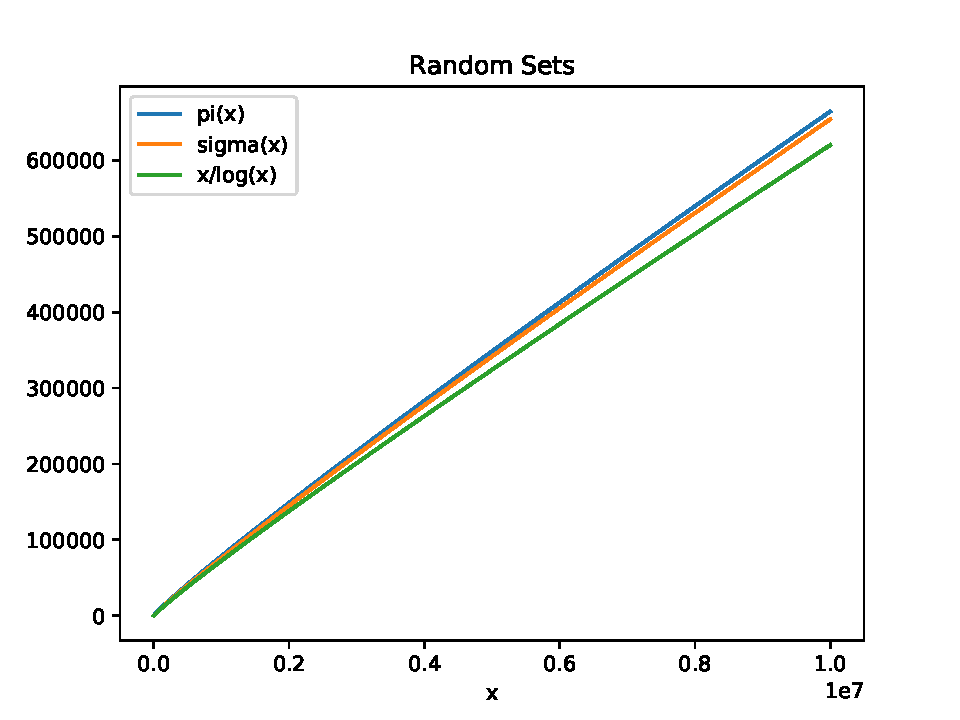
\includegraphics[width = \textwidth]{approche_analytique_sets.pdf}}
\caption{Graphes de $\sigma(x)$, $\pi(x)$ et $\frac{x}{\log(x)}$ }
	\label{im:image1}
\end{figure}

\subsubsection{Écart entre $\pi(x)$ et $\sigma(x)$}

La fonction $\sigma$ semble suivre la même allure que $\pi(x)$. Cependant, lors de nos expérimentations, nous avons
dessinés des graphes (que vous trouverez en annexe) pour des valeurs de $x$ inférieures à celles de la figure \ref{im:image1}. Pour des petites valeurs de $x$, la courbe de $\sigma$ était presque confondue avec celle de $\frac{x}{\log(x)}$. Lorsque les valeurs de $x$ sont de plus en plus grandes, $\sigma(x)$ tend vers $\pi(x)$. Pour analyser l'écart entre $\pi(x)$ et $\sigma(x)$, nous avons tracé le graphe de la fonction $\frac{\pi(x)}{\sigma(x)}$ : 

\hspace{1cm}

La figure \ref{im:image2} devrait apparaitre ici.
\begin{figure}[htbp]
	\centerline{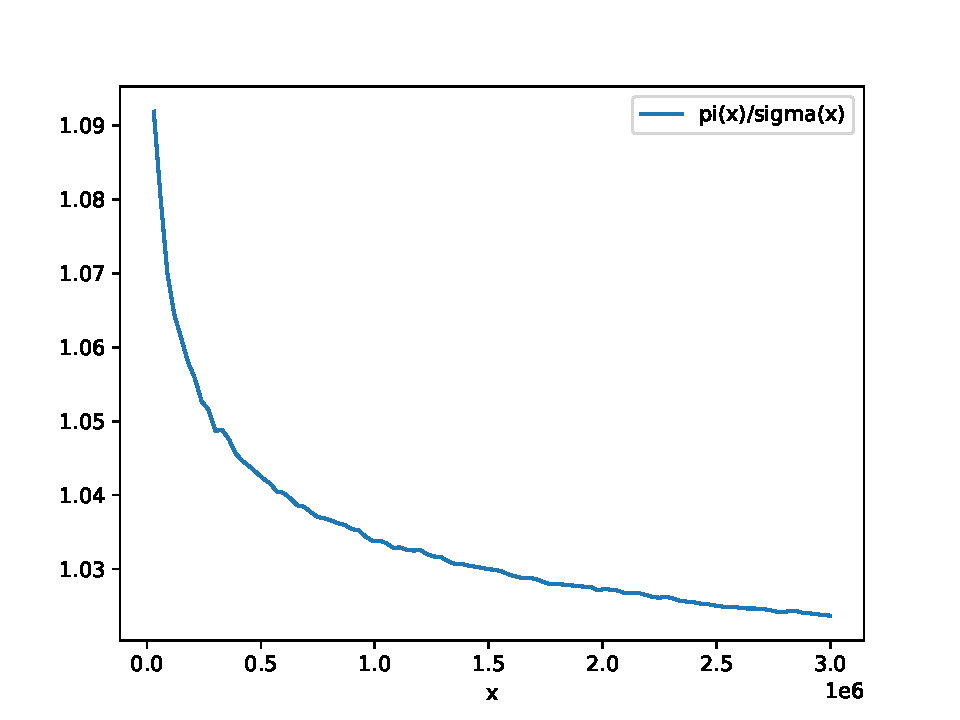
\includegraphics[width = \textwidth]{ecarts.pdf}}
\caption{Graphe de $\frac{\pi(x)}{\sigma(x)}$ }
	\label{im:image2}
\end{figure}
On peut en conclure que $ \pi(x) \sim \sigma(x) $.


\subsubsection{Le Théorème des Nombres Premiers}

L'objectif de cette section est de prouver la fidélité de nos ensembles aléatoires $Q$ à la répartition des nombres premiers.
Pour ce faire, nous allons vérifier si le Théorème des Nombres Premiers, cité ci-après, est vrai quand on remplace $\pi(x)$ par $\sigma(x)$. 

\begin{Thm}[Théorème des Nombres Premiers]
\label{TNP}
	Quand $x$ tend vers l'infini : 
	\[ \pi(x) \sim \frac{x}{\log(x)}  \]
\end{Thm}

Pour démontrer le Théorème des Nombres Premiers, il a été démontré que, quand $x$ tend vers l'infini, $ Li(x) \sim \frac{x}{\log(x)} $. Nous pouvons montrer, graphiquement, que lorsque $x$ tend vers l'infini, $ \sigma(x) \sim Li(x) $ (voir figure \ref{im:image3}), ce qui implique que $ \sigma(x) \sim \frac{x}{\log(x)} $.
\begin{figure}[htbp]
	\centerline{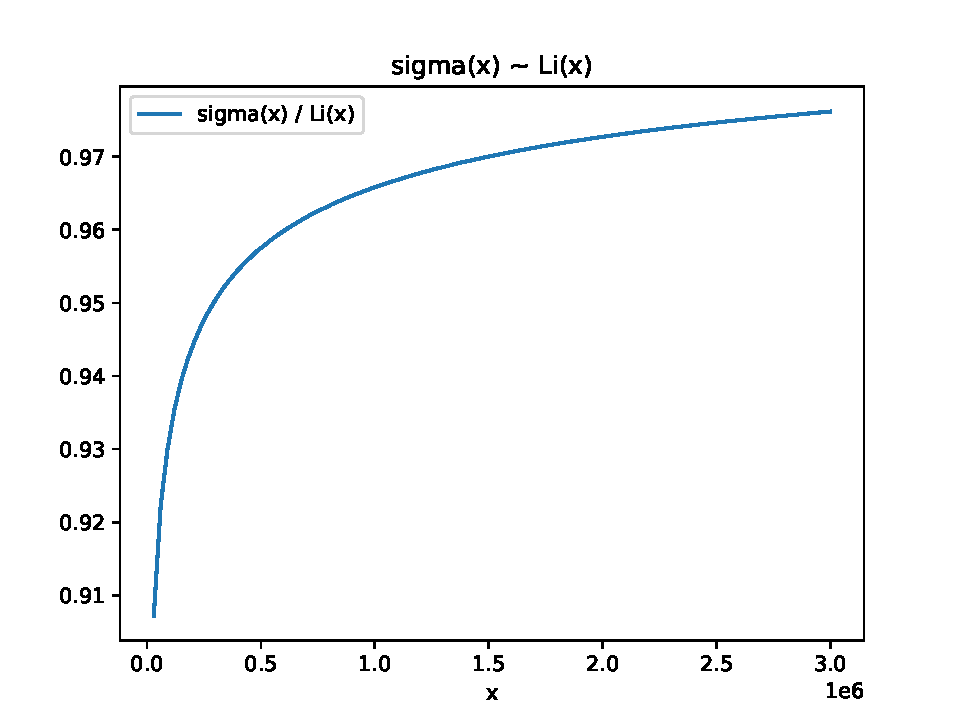
\includegraphics[width = \textwidth]{test2.pdf}}
\caption{Graphe de $\frac{\sigma(x)}{Li(x)}$ }
	\label{im:image3}
\end{figure}



\end{document}







